\scanpage{40}

On en conclut un isom canonique
\reversemarginpar
\margin{Cet isomorphisme\\
reste-t-il valable\\
pour $X$ singulier ???\\
Il est possible\\
qu'on ait\\
besoin de\\
$H^i(X,G_m)=0$\\
pour $i\geqslant2$, qui\\
\unsure{doit} tenir \unsure{si|de}\\
$X$ non sing ??}
\normalmarginpar
\begingroup
\setbox0=\hbox{$\displaystyle H^1(X,A)\xleftarrow{\sim}\operatorname{Ext}^1(A',\underline{\operatorname{Pic}}_X)$}
\ht0=\dimexpr\ht0+9pt\relax
\dp0=\dimexpr\dp0+9pt\relax
\begin{center}
\leavevmode
\rlap{\begin{tikzpicture}[overlay,baseline=0pt]
\draw (-3pt,\ht0) -- (\dimexpr\wd0+3pt\relax,\dimexpr\ht0+1pt\relax);
\draw (-7pt,\dimexpr\ht0-4pt\relax) -- (-7pt,-\dp0) -- (\dimexpr\wd0+4pt\relax,-\dp0) -- (\dimexpr\wd0+3pt\relax,\dimexpr-\dp0+2pt\relax);
\draw (\dimexpr\wd0+7pt\relax,\dimexpr\ht0-4pt\relax) -- (\dimexpr\wd0+7pt\relax,\dimexpr-\dp0+4pt\relax) -- (\dimexpr\wd0+6pt\relax,\dimexpr-\dp0+5pt\relax);
\end{tikzpicture}}
\usebox0
\end{center}
\endgroup

($A$, variété abelienne), qu'on comparera à la
formule de dualité
\begingroup
\setbox0=\hbox{$\displaystyle H^1(X,G)\simeq\operatorname{Hom}(D(G),\underline{\operatorname{Pic}}_X)$}
\ht0=\dimexpr\ht0+9pt\relax
\dp0=\dimexpr\dp0+9pt\relax
\begin{center}
\leavevmode
\rlap{
\begin{tikzpicture}[overlay,baseline=0pt]
\draw (-3pt,\ht0) -- (\dimexpr\wd0+9pt\relax,\dimexpr\ht0+1pt\relax);
\draw (-7pt,\dimexpr\ht0-6pt\relax) -- (-7pt,\dimexpr-\dp0+5pt\relax);
\draw (-9pt,-\dp0) -- (\dimexpr\wd0+3pt\relax,\dimexpr-\dp0+2pt\relax) -- (\dimexpr\wd0+3pt\relax,\dimexpr-\dp0+3pt\relax);
\draw (\dimexpr\wd0+7pt\relax,\dimexpr\ht0-12pt\relax) -- (\dimexpr\wd0+7pt\relax,\dimexpr-\dp0+5pt\relax);
\end{tikzpicture}}
\usebox0
\end{center}
\endgroup
pour $G$ commutatif \unsure{affine|ffine}.

Remarque, On a des hom canoniques
\diagram{\begin{tikzcd}[ampersand replacement=\&,column sep=large,row sep=large]
\operatorname{Ext}^1(\underline{\operatorname{Alb}}_X,A) \arrow[r] \arrow[d,"\wr"] \& H^1(X,A)\\
\operatorname{Ext}^1(A',\underline{\operatorname{Alb}}_X') \arrow[d,"\unsure{\wr}"] \&\\
\operatorname{Ext}^1(A',\underline{\operatorname{Pic}}^\tau) \&
\end{tikzcd}}

dont on voit que c'est des \uline{isomorphismes}
d\uline{onc}, qui définissent sur les \unsure{trois} groupes
en question l'isomorphisme envisagé plus haut.
\reversemarginpar
\margin{39}
\normalmarginpar
